\documentclass[a4paper]{scrartcl}
\usepackage[utf8]{inputenc}
\usepackage[english]{babel}
\usepackage{graphicx}
\usepackage{lastpage}
\usepackage{pgf}
\usepackage{wrapfig}
\usepackage{hyperref}
\usepackage{fancyvrb}
\usepackage{fancyhdr}
\usepackage{float}
\pagestyle{fancy}

% Create header and footer
\headheight 27pt
\pagestyle{fancyplain}
\lhead{\footnotesize{Internet Applications, ID1354}}
\chead{\footnotesize{Name of the Report}}
\rhead{}
\lfoot{}
\cfoot{\thepage\ (\pageref{LastPage})}
\rfoot{}

% Create title page
\title{Name of the Report}
\subtitle{Internet Applications, ID1354}
\author{Your Name and Email Address}
\date{Date}

\begin{document}

\maketitle

\section*{Tips for Report Writing}
\textbf{REMOVE THIS SECTION BEFORE SUBMITTING THE REPORT.}\\

\noindent \textit{The target audience has exactly the same skills as the author, except they do not know anything at all about the specific program described in the report.} \\

Consider the following:

\begin{itemize}
  \item \textbf{The report must be \textit{centered around the requirements}. Which are they (Introduction), how did you work to meet them (Method), what is the solution that meets them (Result), and how can you be sure they are met (Discussion). This is the IMRaD method.}

  \item \textbf{The report must show that you have done the work yourself and that you have understood what you have done. Both of these goals are met by carefully explaining the source code.}

  \item Is spelling and grammar correct? Is spoken language avoided?

  \item Does the report have a good structure with sections, subsections and paragraphs?

  \item Is the solution clearly explained? Will the reader understand the program? What would you yourself want to know if you read about the program, is that included in the report?

  \item Is the solution analyzed and evaluated? Are important properties of the program explained? Should there have been more extensive evaluation?

  \item Is the text clarified with images and/or other figures, and with links to the code in your Git repository? Remember that all figures (images, tables, graphs, code listings, etc) shall be numbered and have a short explaining text.
\end{itemize}

\section{Introduction}

\noindent
The task was to use PHP to store data permanently on the server, and demo this functionality,
by storing users, comments, and this solution went as far as storing recipes as well.
Users and comments had to be stored on the server and could not be hardcoded.
\section{Literature Study}
I was already quite familiar with PHP, Javascript, JSON, and PostgreSQL, specific
commands for PHP and the PostgreSQL API was read up on, as well as some 
PHP functionality, mostly on PHP.net.

\section{Method}

\noindent
As I already had a good grasp on what needed to be done, the first step in building the solution was to pick the tech-stack,
the solution is implemented using Nginx, PHP, Javascript with AJAX calls, and the database backend
is PostgreSQL, as PHP and Javascript is demanded by the course, the only remaining question in the tech-stack,
would be what database and webserver to use,
I chose PostgreSQL and Nginx, both are open source, scalable, and PostgreSQL for example provide a lot of benefit over,
MySQL/MariaDB, one of those benefits being JSON fields.
\\\\
Again the website started out with a simple login form
using HTML/CSS/PHP/Javascript/SQL, and
code that adhered to the requirements, then the development
occured iteratively, adding more and more elements to make
sure the login form looked natural on the website.
\begin{center}
    \begin{tabular}{  l | r }
    Tool & Choice \\ 
    \hline
    Editor & \textit{Vim}\\
    Version Control & \textit{Git - Github}\\
    Web Server & \textit{nginx}\\
    Database & \textit{PostgreSQL 10.5-1}\\
    PHP & \textit{7.2.10-1} \\
    \end{tabular}
\end{center}
\noindent
\section{Result}

\begin{figure}[H]
  \begin{center}
    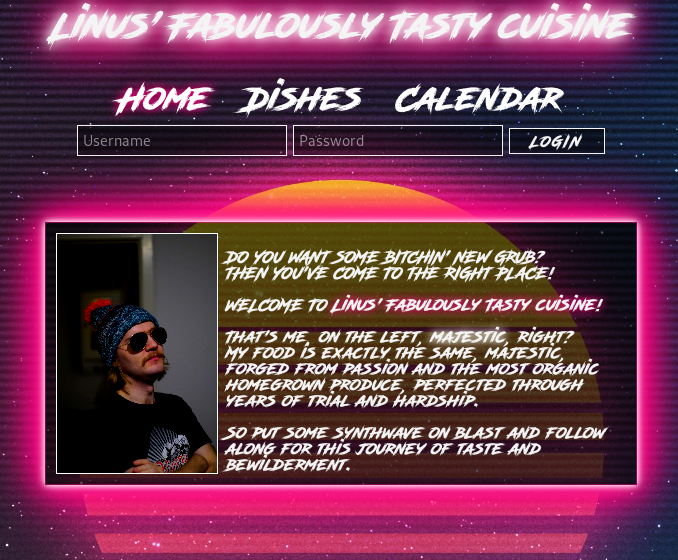
\includegraphics[scale=0.3]{images/login.png}
    \caption{Login, as show on every page.}
    \label{fig:login}
  \end{center}
\end{figure}

\begin{figure}[H]
  \begin{center}
    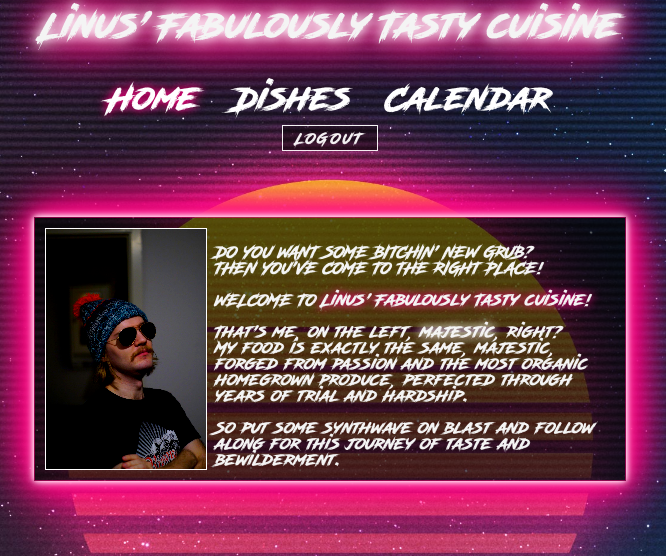
\includegraphics[scale=0.3]{images/logout.png}
    \caption{Logout, as show on every page while logged in.}
    \label{fig:logout}
  \end{center}
\end{figure}

\textbf{\href{https://github.com/linus-dev/KTH-Projects/tree/master/ID1354/2}{Github}}\\\\

\noindent
The solution was a simple login form below the nav bar as
seen in \ref{fig:login} upon logging in, the login form is
switched to the logout as seen in \ref{fig:logout}. Both
of these are displayed on every page to make sure the
user has an easier time logging in or logging out, without
having to redirect themselves to another page.
\\\\
It is important that the login/logout form follows the 5 basic heuristics of
interface design.
\begin{itemize}
\item{Visibility of system status}\\
  The user quite easily can distinguish between begin logged in and logged out,
  there is no dependencies on colours et cetera, so the system status should be
  easily visible to any user.
\item{Match between system and the real world}\\
  There was not a lot text, however the UI speaks for itself, and login/logout
  are quite universal in today's society and easily understood by any user, username and password is also displayed in
  textboxes accordingly.
\item{Consistency and standards}\\
  The login and logout forms are consistent throughout all pages, it remains in
  the same place at all times, and it also conforms to common login form standards,
  such as having a normal username and password form.
\item{Recognition rather than recall}\\
  The users always know if they are logged in or logged out on every page at the same
  location.
\item{Aesthetic and minimalist design}\\
  The login and logout are by all means minimal and fits the aesthetic style of the rest of the website.
\end{itemize}

\begin{figure}[H]
  \begin{center}
    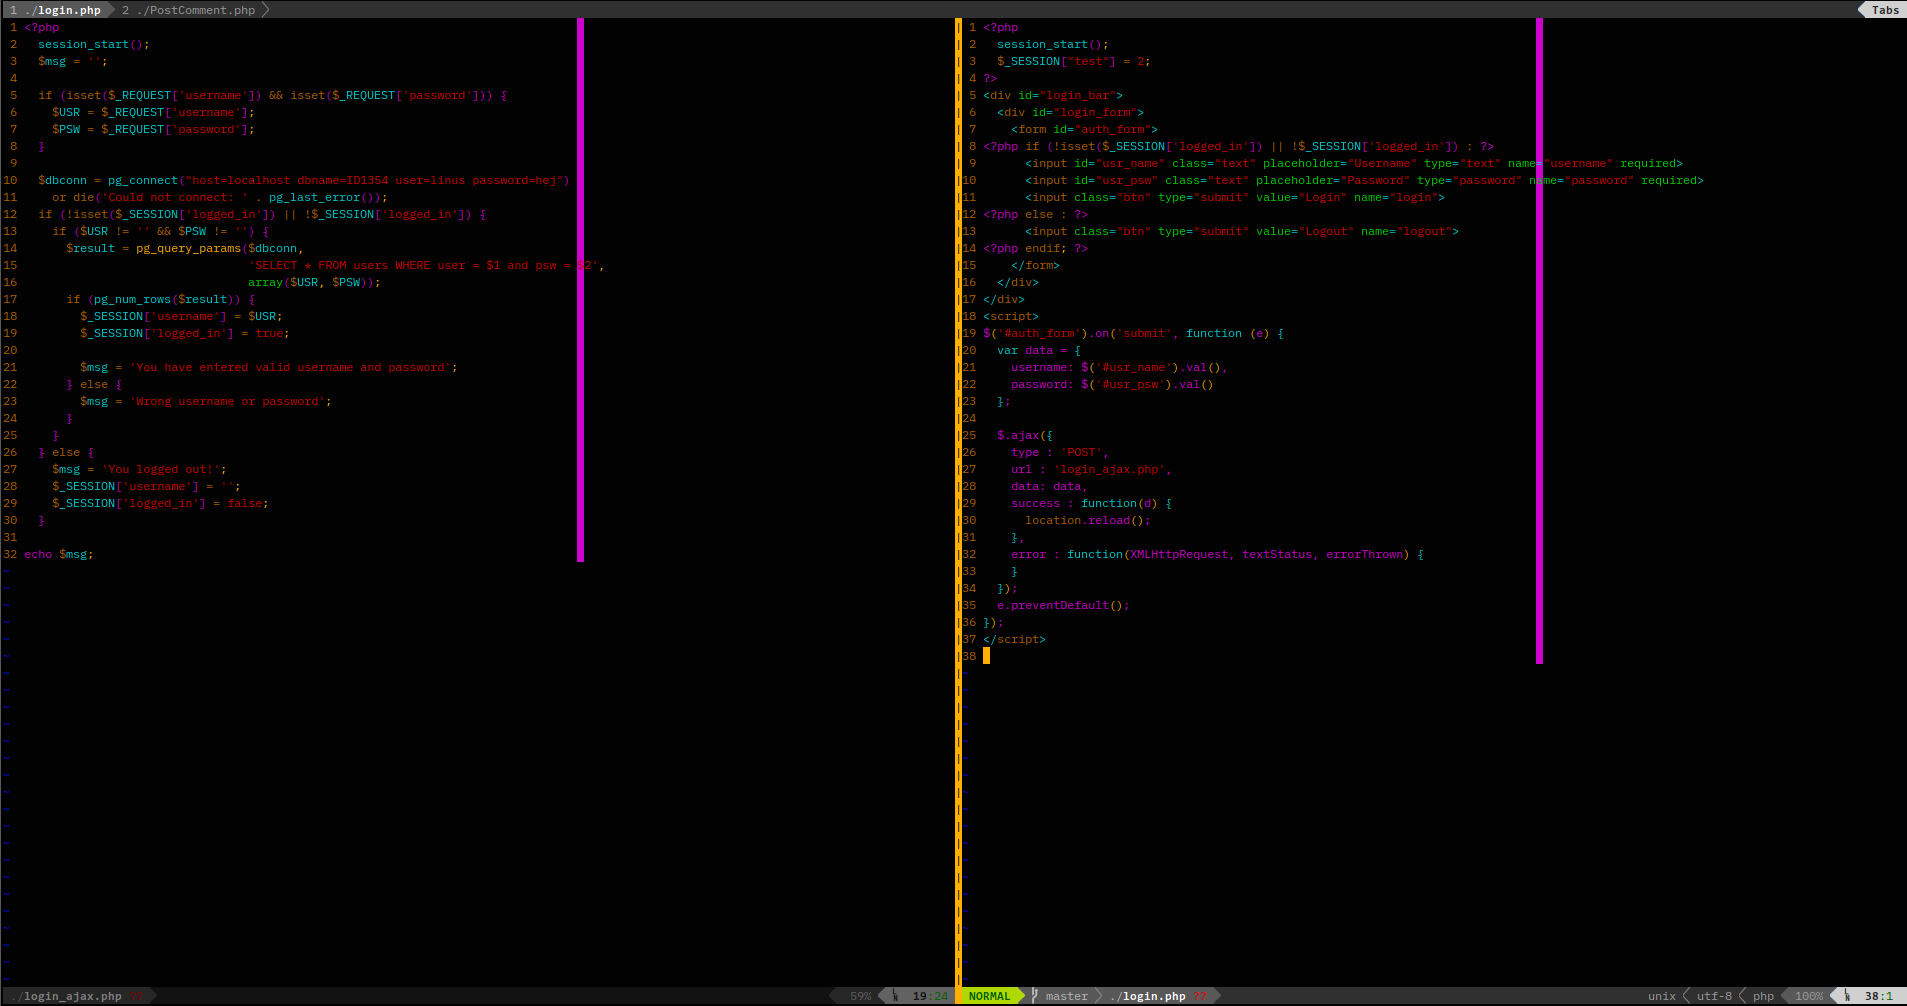
\includegraphics[scale=0.32]{images/login_code.png}
    \caption{login.php and login\_ajax.php}
    \label{fig:login_code}
  \end{center}
\end{figure}
The login form utilises AJAX and PHP to perform both the login and logout.

\section{Discussion}

\textbf{This section \textit{analysis} the result presented in the previous section.} \\

\noindent Summarize the requirements and \textit{clearly state which of them you have met}. What lessons have you learned and what problems did you face? How were the problems solved? Should you have done something differently?

\section{Comments About the Course}

Any comment(s) related to this course offering or to coming offerings is much appreciated. \textit{Please also tell approximately how much time you spent on the assignment}, including lectures and exercises. This is of great help for course evaluation.

\end{document}
